\documentclass[10pt]{article}
\usepackage[spanish]{babel}
\usepackage[utf8]{inputenc}
\usepackage[T1]{fontenc}
\usepackage{amsmath}
\usepackage{amsfonts}
\usepackage{amssymb}
\usepackage[version=4]{mhchem}
\usepackage{stmaryrd}
\usepackage{graphicx}
\usepackage[export]{adjustbox}
\graphicspath{ {./images/} }
\usepackage{bbold}

\begin{document}
\section*{Construcción}
\section*{1. Criptografía.}
Supongamos que Juan quiere enviar un mensaje a Pedro de forma tal que únicamente Pedro sea capaz de entender su contenido. Una manera ingenua de hacer esto es reemplazar cada letra, signo de puntuación, espacio, etc. del mensaje original por un número de dos cifras, según una tabla de conversión convenida previamente entre Juan y Pedro que sólo ellos dos conocen. De esta manera Juan, utilizando la tabla, convierte el texto en un número y se lo envía a Pedro, quien recupera el mensaje original utilizando a su vez la tabla de conversión.\\
Por ejemplo, si el mensaje fuese ESTO ES UN SECRETO y utilizamos la tabla de conversión

\begin{center}
\begin{tabular}{|c|c|c|c|c|c|c|c|c|c|c|c|c|c|c|c|c|c|c|}
\hline
A & B & C & D & E & F & G & H & I & J & K & L & M & N & O & P & Q & R & S \\
\hline
01 & 02 & 03 & 04 & 05 & 06 & 07 & 08 & 09 & 10 & 11 & 12 & 13 & 14 & 15 & 16 & 17 & 18 & 19 \\
\hline
\end{tabular}
\end{center}

\begin{center}
\begin{tabular}{|c|c|c|c|c|c|c|c|}
\hline
T & U & V & W & X & Y & Z & espacio \\
\hline
20 & 21 & 22 & 23 & 24 & 25 & 26 & 00 \\
\hline
\end{tabular}
\end{center}

el número que recibiría Pedro sería 051920150005190021140019050318052015\\
Sin embargo, esta no es una manera segura ya que es posible descifrar el mensaje comparando la frecuencia con la que aparece cada uno de los números de dos cifras con la frecuencia estadística que tiene cada letra. Por ejemplo, que el número 05 aparezca más veces que cualquier otro indica que probablemente sea una A o una E (que son las letras que más frecuentemente aparecen en cualquier texto).\\
Veamos otras formas más seguras de enviar mensajes. La idea general es aplicar al mensaje una cierta transformación (es decir, encriptarlo) de forma tal que ningún intruso que intercepte el mensaje encriptado sea capaz de aplicarle la transformación inversa. Observemos que la transformación inversa debe ser mantenida en secreto siempre, mientras que la que encripta puede ser tanto pública como privada. Esto se debe a que existen ciertas funciones, llamadas de una sola vía, que son sencillas de evaluar pero cuya inversa es muy difícil de determinar. Por lo tanto, si la transformación que se utiliza para encriptar es de una sola vía, no es necesario que sea mantenida en secreto.

Claves privadas. En este caso la transformación que encripta el mensaje utiliza una clave que sólo es conocida por Juan y Pedro. Unicamente quienes conozcan la clave son capaces de encriptar el mensaje. De esta manera, cuando Juan envía a Pedro un mensaje encriptado utilizando la clave que ambos convinieron previamente y que sólo ellos conocen, Pedro sabe con certeza que el mensaje proviene de Juan ya que nadie más podría ser capaz de\\
encriptarlo. Veamos ahora un ejemplo que tiene la particularidad de que la transformación que se utiliza para encriptar es la misma que la que se utiliza para desencriptar. Es decir, en este ejemplo, la transformación que encripta coincide con su inversa. Esta clase de transformaciones se denominan involuciones.\\
En primer lugar, Juan y Pedro eligen como clave un string de 30 dígitos binarios (es decir, tal que cada dígito sea cero o uno) que mantienen en secreto. Supongamos que la clave elegida sea

$$
101000110110101100101101001011
$$

Ahora, Juan convierte el mensaje en un string de dígitos binarios reemplazando cada letra por un string de cinco dígitos binarios según una tabla de conversión previamente acordada con Pedro. Por ejemplo, la tabla de conversión puede obtenerse de la tabla

\begin{center}
\begin{tabular}{|c|c|c|c|c|c|c|c|c|c|c|c|c|c|c|c|c|c|c|}
\hline
A & B & C & D & E & F & G & H & I & J & K & L & M & N & O & P & Q & R & S \\
\hline
01 & 02 & 03 & 04 & 05 & 06 & 07 & 08 & 09 & 10 & 11 & 12 & 13 & 14 & 15 & 16 & 17 & 18 & 19 \\
\hline
\end{tabular}
\end{center}

\begin{center}
\begin{tabular}{|c|c|c|c|c|c|c|c|}
\hline
T & U & V & W & X & Y & Z & espacio \\
\hline
20 & 21 & 22 & 23 & 24 & 25 & 26 & 00 \\
\hline
\end{tabular}
\end{center}

reemplazando cada número de dos cifras por su representación en base 2. De esta manera, cada letra S del mensaje original será reemplazada por el string 10011, ya que esta es la representación de 19 en base 2 . Luego de reemplazar cada letra por su correspondiente string de cinco dígitos binarios, Juan parte el string total obtenido en bloques de 30 dígitos binarios cada uno. Ahora nuestro mensaje se ha convertido en

$$
\begin{aligned}
& \text { bloque 1: } \underbrace{00101}_{E} \underbrace{10011}_{S} \underbrace{10100}_{T} \underbrace{01111}_{O} \underbrace{00000}_{\text {espacio }} \underbrace{00101}_{E} \\
& \text { bloque 2: } \underbrace{10011}_{S} \underbrace{00000}_{\text {espacio }} \underbrace{10101}_{U} \underbrace{01110}_{N} \underbrace{00000}_{\text {espacio }} \underbrace{10011}_{S} \\
& \text { bloque 3: } \underbrace{00101}_{E} \underbrace{00011}_{C} \underbrace{10010}_{R} \underbrace{00101}_{E} \underbrace{10100}_{T} \underbrace{01111}_{O}
\end{aligned}
$$

A continuación, Juan transforma, utilizando la clave, cada uno de estos bloques (que llamaremos bloques originales) en un nuevo bloque binario (que llamaremos bloques transformados) poniendo un cero en el $i$-ésimo lugar del bloque transformado si el $i$-ésimo dígito de la clave coincide con el $i$-ésimo dígito del bloque original y poniendo un uno en otro caso.\\
Por ejemplo, en nuestro caso el primer dígito del bloque 1 original es 0 y el primer dígito de la clave es 1 . Como no coinciden, el primer dígito del bloque transformado será 1. Análogamente, el segundo dígito del bloque 1 original es 0 y el segundo dígito de la clave es 0 . Como coinciden, el segundo dígito del bloque transformado será 0 .\\
bloque 1 original: 001011001110100011110000000101\\
clave: 101000110110101100101101001011\\
bloque 1 transformado: 100011111000001111011101001110\\
Ahora hacemos lo mismo con los restantes dos bloques:\\
bloque 2 original: 100110000010101011100000010011\\
clave: 101000110110101100101101001011\\
bloque 2 transformado: 001110110100000111001101011000\\
bloque 3 original: 001010001110010001011010001111\\
clave: 101000110110101100101101001011\\
bloque 3 transformado: 100010111000111101110111000100\\
Finalmente, Juan envía a Pedro los bloques transformados.\\
Para desencriptar el mensaje, Pedro efectua en cada bloque recibido la misma operación, es decir, utilizando la clave reconstruye los bloques originales comparando el $i$-ésimo dígito del bloque transformado con el $i$-ésimo dígito de la clave. Si estos coinciden significa que el $i$-ésimo dígito del bloque original era un cero y si no coinciden que era un uno. Para ejemplificar, desencriptemos el segundo bloque:\\
bloque 2 transformado: 001110110100000111001101011000\\
clave: 101000110110101100101101001011\\
bloque 2 original: 100110000010101011100000010011\\
Por último, Pedro descifra el mensaje reemplazando cada string de cinco dígitos binarios por la correspondiente letra según la tabla de conversión.

La ventaja de este sistema radica en que una misma letra puede resultar transformada en diferentes strings según sea su ubicación en el texto. Por ejemplo, la primera E de nuestro mensaje (representada por los primeros cinco dígitos del bloque 1) se transformó en 10001 (primeros cinco dígitos del bloque 1 transformado), la segunda (representada por los últimos cinco dígitos del bloque 1) en 01110 (últimos cinco dígitos del bloque 1 transformado), la tercera en 10001 y la cuarta en 10111. También, la primera S se transformó en 11110, la segunda en 00111 y la tercera en 11000. Además, diferentes letras pueden resultar transformadas en el mismo string. Por ejemplo, tanto la segunda E como la C se transformaron en 01110 . Esto hace que sea prácticamente imposible desencriptar el mensaje sin conocer la clave. En este caso, la cantidad de posibles claves de 30 dígitos binarios es $2^{30}$ pero está claro que para mensajes más largos podríamos partir el mensaje binario original en bloques de 100 dígitos y, por lo tanto, utilizar claves de 100 dígitos\\
binarios. En tal caso la cantidad de posibles claves sería enorme ( $2^{100}$ ) lo que hace que ninguna persona que no conozca la clave pueda determinarla por ensayo y error (es decir, probando con cada posible clave hasta obtener un texto coherente).\\
Como vemos, la seguridad de este método radica en la privacidad de la clave. Nos preguntamos entonces cómo pueden hacer Juan y Pedro para acordar una clave con total certeza de que sólo ellos la conozcan. Obviamente, la manera más segura es acordar una clave sin tener que transmitirla, ya que al transmitirla se corre el riesgo de que alguien la intercepte. El siguiente método, ideado por W. Diffie y M. Hellman, logra este objetivo: primero, Juan y Pedro eligen un número primo $p$ y un entero $a$ coprimo con $p$ tal que $r_{p}\left(a^{j}\right) \neq 1$ para todo $1 \leq j<p-1$. Un tal entero $a$ se llama una raíz primitiva módulo $p$ (observemos que para cualquier primo $p$ siempre existe al menos una raíz primitiva módulo $p$ ). Tanto $p$ como $a$ no necesitan guardarse en secreto, sino que pueden ser conocidos por cualquier persona. Luego Juan elige un número natural $k$ menor que $p-1$ y tal que $a^{k}>p$ y, a su vez, Pedro elige un número natural $r$ menor que $p-1 \mathrm{y}$ tal que $a^{r}>p$. Los números $k \mathrm{y} r$ son secretos, $k$ es conocido sólo por Juan y $r$ es conocido sólo por Pedro. Juan envía a Pedro el número $b=r_{p}\left(a^{k}\right)$ y Pedro envía a Juan el número $c=r_{p}\left(a^{r}\right)$. Entonces Juan calcula $r_{p}\left(c^{k}\right)$ y Pedro calcula $r_{p}\left(b^{r}\right)$.\\
Como $c \equiv a^{r}(p)$ entonces $c^{k} \equiv\left(a^{r}\right)^{k}=a^{r k}(p)$. Del mismo modo, como $b \equiv a^{k}(p)$ entonces $b^{r} \equiv\left(a^{k}\right)^{r}=a^{r k}(p)$. Luego, $c^{k} \equiv b^{r}(p)$, de donde $r_{p}\left(c^{k}\right)=r_{p}\left(b^{r}\right)$. Este número $r_{p}\left(c^{k}\right)=r_{p}\left(b^{r}\right)$, que tanto Juan como Pedro conocen pero que nunca fue transmitido, será la clave acordada. Observemos que si lo que quisieran es una clave binaria, basta tomar entonces la representación en base 2 de $r_{p}\left(c^{k}\right)=r_{p}\left(b^{r}\right)$.\\
Para fijar ideas, supongamos que el primo convenido entre Juan y Pedro sea $p=127$ y que la raíz primitiva módulo $p$ sea $a=3$ (dejamos a cargo del lector verificar que 127 es primo y que 3 es una raíz primitiva módulo 127). Supongamos además que Juan elige $k=16$ y Pedro elige $r=30$ y veamos cómo hacen Juan y Pedro para obtener la clave. Primero, Juan calcula $b=r_{p}\left(a^{k}\right)=r_{127}\left(3^{16}\right)=71$ y se lo envía a Pedro y Pedro calcula $c=r_{p}\left(a^{r}\right)=r_{127}\left(3^{30}\right)=38$ y se lo envía a Juan. Luego, como Juan conoce $c=38$ y $k=16$, puede calcular $r_{p}\left(c^{k}\right)=r_{127}\left(38^{16}\right)=76$. Análogamente, como Pedro conoce $b=71$ y $r=30$, puede calcular $r_{p}\left(b^{r}\right)=r_{127}\left(71^{30}\right)=76$. Por lo tanto, la clave acordada (que es conocida por ambos pero que nunca fue transmitida) es 76 . Si quisieran una clave binaria, podrían tomar, por ejemplo, la representación en base 2 de 76 que es 1001100.\\
En la realidad, el primo $p$ elegido es un número de muchísimas más cifras. Esto produce, por un lado, que la clave resulte un número de muchas más cifras (cosa que ya vimos que es conveniente) y, por otro, que el método sea seguro ya que cuando $p$ es un primo muy grande y $a$ es una raíz primitiva módulo $p$ entonces no existe ningún método eficiente que permita calcular $k$ a partir de $p, a$ y $r_{p}\left(a^{k}\right) \mathrm{y}$, por lo tanto, si un intruso interceptara la comunicación entre Juan y Pedro y lograra conocer $b=r_{p}\left(a^{k}\right)$ y $c=r_{p}\left(a^{r}\right)$, no pudiendo determinar $k$ y $r$ le sería imposible calcular la clave.

Finalmente, veamos cómo pueden hacer Juan y Pedro para determinar $b, c$ y la clave rápidamente. Juan necesita calcular $b=r_{127}\left(3^{16}\right)$ y $r_{127}\left(38^{16}\right)$. Esto lo puede hacer de la siguiente manera:


\begin{align*}
& 3^{2^{0}}=3^{1}=3 \equiv 3 \\
& 3^{2^{1}}=3^{2^{0} \cdot 2}=(127)  \tag{127}\\
& \left.\left.3^{2^{2}}=3^{2^{0}}\right)^{2}\right) \equiv 3^{2}=9  \tag{127}\\
& \left.3^{2^{3}}=3^{2^{2} \cdot 2}=\left(3^{2^{1}}\right)^{2}\right) \equiv 9^{2}=81  \tag{127}\\
& \left.\left.3^{2^{4}}=3^{2^{2}}\right)^{2}\right) \equiv 81^{2}=6561 \equiv 84  \tag{127}\\
& \left.\left.38^{2^{0}}=38^{2^{3}}\right)^{2}\right) \equiv 84^{2}=7056 \equiv 71  \tag{127}\\
& \left.38^{2^{1}}=38^{2^{0} \cdot 2}=\left(38^{2^{0}}\right)^{2}\right) \equiv 38^{2}=1444 \equiv 47  \tag{127}\\
& \left.38^{2^{2}}=38^{2^{1} \cdot 2}=\left(38^{2^{1}}\right)^{2}\right) \equiv 47^{2}=2209 \equiv 50  \tag{127}\\
& \left.38^{2^{3}}=38^{2^{2} \cdot 2}=\left(38^{2^{2}}\right)^{2}\right) \equiv 50^{2}=2500 \equiv 87  \tag{127}\\
& \left.38^{2^{4}}=38^{2^{3} \cdot 2}=\left(38^{2^{3}}\right)^{2}\right) \equiv 87^{2}=7569 \equiv 76 \tag{127}
\end{align*}


Como $16=2^{4}$, entonces Juan obtiene que $b=r_{127}\left(3^{16}\right)=r_{127}\left(3^{2^{4}}\right)=71$ y la clave es $r_{127}\left(38^{16}\right)=r_{127}\left(38^{2^{4}}\right)=76$.\\
A su vez, Pedro necesita calcular $c=r_{127}\left(3^{30}\right)$ y $r_{127}\left(71^{30}\right)$. Ahora el exponente, 30, no es una potencia de 2. Sin embargo, puede proceder de manera similar, hallando primero el desarrollo en base 2 de 30 , que es 11110 . Esto significa que $30=1.2^{4}+1.2^{3}+1.2^{2}+1.2^{1}+0.2^{0}$ y, por lo tanto,

$$
3^{30}=3^{2^{4}+2^{3}+2^{2}+2^{1}}=3^{2^{4}} \cdot 3^{2^{3}} \cdot 3^{2^{2}} \cdot 3^{2^{1}}
$$

y

$$
71^{30}=71^{2^{4}+2^{3}+2^{2}+2^{1}}=71^{2^{4}} \cdot 71^{2^{3}} \cdot 71^{2^{2}} \cdot 71^{2^{1}}
$$

con lo cual Pedro puede calcular $c$ y la clave de la siguiente manera:


\begin{align*}
& 3^{2^{0}}=3^{1}=3 \equiv 3  \tag{127}\\
& 3^{2^{1}}=3^{2^{0} \cdot 2}=(127)  \tag{127}\\
& \left.\left.3^{2^{2}}=3^{2^{1}}\right)^{2} \cdot 2=\left(3^{2^{1}}\right)^{2}\right) \equiv 3^{2}=9  \tag{127}\\
& 3^{2^{3}}=3^{2^{2} \cdot 2}=(127)  \tag{127}\\
& \left.\left.3^{2^{4}}=3^{2^{2}}\right)^{2}\right) \equiv 81^{2}=6561 \equiv 84  \tag{127}\\
& \left.=3^{2^{3} \cdot 2}=\left(3^{2^{3}}\right)^{2}\right) \equiv 84^{2}=7056 \equiv 71
\end{align*}



\begin{align*}
& 71^{2^{0}}=71^{1}=71 \equiv 71 \\
& \left.71^{2^{1}}=71^{2^{0} \cdot 2}=\left(71^{2^{0}}\right)^{2}\right) \equiv 71^{2}=5041 \equiv 88  \tag{127}\\
& \left.71^{2^{2}}=71^{2^{1} \cdot 2}=\left(71^{2^{1}}\right)^{2}\right) \equiv 88^{2}=7744 \equiv 124  \tag{127}\\
& \left.71^{2^{3}}=71^{2^{2} \cdot 2}=\left(71^{2^{2}}\right)^{2}\right) \equiv 124^{2}=15376 \equiv 9  \tag{127}\\
& \left.71^{2^{4}}=71^{2^{3} \cdot 2}=\left(71^{2^{3}}\right)^{2}\right) \equiv 9^{2}=81 \tag{127}
\end{align*}


Luego,


\begin{gather*}
3^{30}=3^{2^{4}+2^{3}+2^{2}+2^{1}}=3^{2^{4}} \cdot 3^{2^{3}} \cdot 3^{2^{2}} \cdot 3^{2^{1}} \equiv 71 \cdot 84 \cdot 81 \cdot 9= \\
=5964 \cdot 729 \equiv 122 \cdot 94=11468 \equiv 38 \quad(127) \tag{127}
\end{gather*}


y


\begin{align*}
71^{30} & =71^{2^{4}+2^{3}+2^{2}+2^{1}}=71^{2^{4}} \cdot 71^{2^{3}} \cdot 71^{2^{2}} \cdot 71^{2^{1}} \equiv 81 \cdot 9 \cdot 124 \cdot 88= \\
& =729 \cdot 10912 \equiv 94 \cdot 117=10998 \equiv 76 \quad(127) \tag{127}
\end{align*}


de donde finalmente obtiene que $c=r_{127}\left(3^{30}\right)=38$ y la clave es $r_{127}\left(71^{30}\right)=76$.\\
Si el lector ya está convencido de que esta manera de acordar una clave es segura, imagine la siguiente situación: un intruso ha "pinchado" la comunicación entre Juan y Pedro de manera tal que cuando Juan o Pedro envían un mensaje quien realmente lo recibe es el intruso. Además, el intruso puede enviar mensajes a Pedro haciéndose pasar por Juan y a Juan haciéndose pasar por Pedro.\\
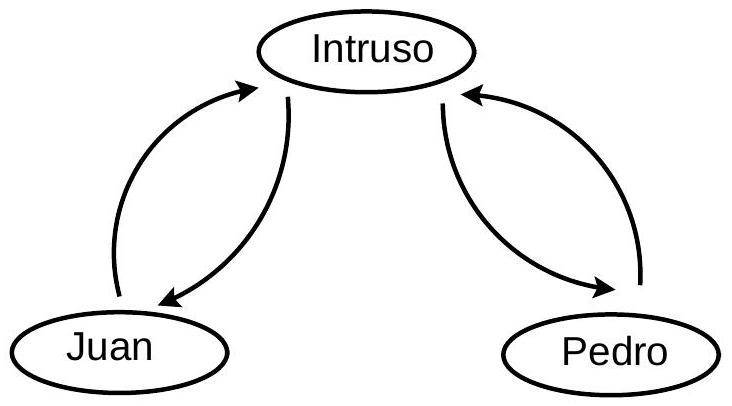
\includegraphics[max width=\textwidth, center]{2025_09_05_76a00afb34b0e185ce5bg-06}

Ahora, cuando Juan envía a Pedro el número $b_{1}=r_{p}\left(a^{k}\right)$ el intruso lo recibe y, haciéndose pasar por Pedro, envía a Juan el número $c_{1}=r_{p}\left(a^{s}\right)$. Ahora ambos calculan la clave $K_{1}=r_{p}\left(c_{1}^{k}\right)=r_{p}\left(b_{1}^{s}\right)$. Por otro lado, el intruso envía a Pedro, haciéndose pasar por Juan, el número $b_{2}=r_{p}\left(a^{t}\right)$ y Pedro envía al intruso, creyendo que es Juan, el número $c_{2}=r_{p}\left(a^{r}\right)$. Finalmente, ambos calculan la clave $K_{2}=r_{p}\left(c_{2}^{t}\right)=r_{p}\left(b_{2}^{r}\right)$. Ahora Juan cree que la clave acordada es $K_{1}$, Pedro cree que es $K_{2}$ y el intruso conoce tanto $K_{1}$ como $K_{2}$. De esta manera, cada vez que Juan le envíe a Pedro un mensaje, el mensaje estará encriptado usando la clave $K_{1}$ y el intruso será quien lo reciba. Entonces el intruso puede desencriptarlo y\\
i) encriptar nuevamente el mensaje pero ahora usando la clave $K_{2}$ y enviárselo a Pedro, quien pensará que proviene de Juan.\\
ii) idem i) pero alterando previamente el contenido del mensaje.\\
iii) no reenviar el mensaje a Pedro y responderle a Juan haciéndose pasar por Pedro usando la clave $K_{1}$.\\
Claramente, lo mismo sucede cuando Pedro envía un mensaje a Juan...\\
Claves públicas. En este caso la transformación que encripta el mensaje utiliza una clave que es de conocimiento público. Cualquier persona tiene acceso a la clave y, por lo tanto, puede encriptar un mensaje. Obviamente, en este caso no puede usarse la misma clave para encriptar y desencriptar, por lo tanto, cada usuario del sistema debe elegir dos claves: una pública, que utilizarán los demás para encriptar los mensajes que le envíen y una privada que sólo él conoce con la cual puede desencriptarlos.\\
Describiremos ahora uno de los sistemas más populares de clave pública, conocido como RSA y creado por Rivest, Shamir y Adleman en 1978 que se basa en el

Teorema de Euler-Fermat: Sea $n$ un número natural y sea $a$ un entero. Si $a$ es coprimo con $n$ entonces $a^{\Phi(n)} \equiv 1(n)$.

En este sistema, cada usuario fabrica dos claves, una pública y una privada, de la siguiente manera: en primer lugar, elige dos primos distintos $p$ y $q$ y calcula su producto $n=p . q$. Luego elige un número natural $e$ menor que $\Phi(n)=(p-1)(q-1)$ y que sea coprimo con $\Phi(n)$ y calcula, utilizando el algoritmo de Euclides, un número natural $d$ tal que e.d $\equiv 1(\Phi(n))$.

El par ( $n, e$ ) constituye la clave pública que permite al resto de los usuarios encriptar los mensajes que le envíen, mientras que la terna ( $p, q, d$ ) debe ser mantenida en secreto y constituye la clave privada que le permitirá desencriptar los mensajes que reciba. En resumen, cada usuario $j$ dispone de una clave pública $\left(n_{j}, e_{j}\right)$ y de una privada $\left(p_{j}, q_{j}, d_{j}\right)$ donde $n_{j}=p_{j} . q_{j}$ y $e_{j} . d_{j} \equiv 1\left(\Phi\left(n_{j}\right)\right)$. Además, todos disponen de una tabla de conversión común para transformar los mensajes en un número antes de encriptarlos.\\
Para enviar un mensaje encriptado a Pedro, cuya clave pública es $(n, e)$, Juan transforma el mensaje en un número utilizando la tabla de conversión y lo parte en bloques de longitud menor que $n$. Luego, para cada bloque $a$, Juan calcula el bloque transformado $b=r_{n}\left(a^{e}\right)$ y se lo envía a Pedro.\\
Para desencriptar cada bloque transformado $b$, Pedro utiliza su clave privada ( $p, q, d$ ) que sólo él conoce y calcula $r_{n}\left(b^{d}\right)$, con lo cual obtiene el bloque original $a$. En efecto, como $e . d \equiv 1(\Phi(n))$, entonces $e . d-1=k \Phi(n)$ para algún $k \in N$. Como $b=r_{n}\left(a^{e}\right) \equiv a^{e}(n)$, se tiene que


\begin{equation*}
b^{d} \equiv\left(a^{e}\right)^{d}=a^{e . d}=a^{1+k \Phi(n)}=a \cdot\left(a^{\Phi(n)}\right)^{k} \tag{n}
\end{equation*}


Veamos que $a \cdot\left(a^{\Phi(n)}\right)^{k} \equiv a(n)$. Esto es claro cuando $a$ es coprimo con $n$ ya que en ese caso $a^{\Phi(n)} \equiv 1 \quad(n)$. Pero también vale si $a$ y $n$ no son coprimos. En efecto, en tal caso se tiene que $a$ es divisible por $p$ o por $q$, pero no por ambos, ya que $n=p . q$ y $a<n$. Supongamos\\
entonces que $a$ es divisible por $p$ y no por $q$. Entonces $a \equiv 0(p)$ y $a^{q-1} \equiv 1(q)$, de donde

$$
a \cdot\left(a^{\Phi(n)}\right)^{k} \equiv 0 \equiv a \quad(p)
$$

y


\begin{equation*}
a \cdot\left(a^{\Phi(n)}\right)^{k} \equiv a \cdot\left(a^{(p-1)(q-1)}\right)^{k}=a \cdot\left(a^{q-1}\right)^{(p-1) k} \equiv a \tag{q}
\end{equation*}


Luego, como $n=p . q$ y $p$ y $q$ son primos distintos, resulta que $a \cdot\left(a^{\Phi(n)}\right)^{k} \equiv a(n)$ de donde $b^{d} \equiv a(n) \mathrm{y}$, como $a$ es un número natural menor que $n$ entonces $a=r_{n}\left(b^{d}\right)$.\\
De esta manera, Pedro recupera cada bloque original y reconstruye el mensaje utilizando la tabla de conversión.\\
Observemos que para poder desencriptar, es necesario conocer $d$, que sólo puede calcularse conociendo $\Phi(n)$. Dado que, para valores de $n$ suficientemente grandes, $\Phi(n)$ no se puede calcular sin conocer la factorización de $n$, la seguridad de este sistema descansa en el hecho de que para factorizar números grandes se requiere muchísimo tiempo. En la realidad, los primos $p$ y $q$ elegidos son números de más de 100 cifras, con lo cual resulta imposible determinar la factorización de $n=p . q$.

Autenticidad del emisor. Como ya observamos antes, cuando se utiliza para encriptar una clave privada la autenticidad del emisor está garantizada: cuando Juan envía a Pedro un mensaje encriptado utilizando una clave que ambos convinieron previamente y que sólo ellos conocen, Pedro sabe con certeza que el mensaje proviene de Juan ya que nadie más podría ser capaz de encriptarlo. En cambio, cuando se utiliza una clave pública esto no sucede. Supongamos que Pedro recibe un mensaje supuestamente enviado por Juan. Debido a que la clave pública de Juan es conocida por todos, Pedro no puede estar seguro de que el mensaje fue realmente enviado por Juan y no por otra persona. Supongamos que $(n, e)$ y $(m, r)$ son las respectivas claves púbicas de Pedro y Juan y que $(p, q, d)$ y $\left(p^{\prime}, q^{\prime}, s\right)$ son las claves privadas. Veamos cómo se puede hacer para garantizar la autenticidad del emisor del mensaje.\\
Supongamos que $n \leq m$. En este caso, Juan transforma el mensaje en un número y lo parte en bloques de longitud menor que $n$. Para encriptar cada bloque $a$, efectúa dos transformaciones: primero una utilizando la clave pública de Pedro y luego otra utilizando su propia clave privada. Para obtener el bloque transformado Juan primero calcula $b=r_{n}\left(a^{e}\right)$, luego calcula $c=r_{m}\left(b^{s}\right)$ y envía $c$ a Pedro. Para desencriptar el bloque transformado, Pedro utiliza la clave pública de Juan y su propia clave privada: calcula primero $r_{m}\left(c^{r}\right)$ que es igual a $b$ pues $c^{r} \equiv b(m)$ y $b<n \leq m$. Una vez obtenido $b$, Pedro calcula $r_{n}\left(b^{d}\right)$ que resulta ser igual a $a$ ya que $b^{d} \equiv a(n)$ y $a<n$.\\
Si, en cambio, $m<n$, Juan transforma el mensaje en un número que ahora parte en bloques de longitud menor que $m$. Ahora, para encriptar cada bloque $a$, realiza las mismas transformaciones que antes pero en orden inverso: primero calcula $b=r_{m}\left(a^{s}\right)$, luego $c=r_{n}\left(b^{e}\right)$. Para desencriptar el bloque transformado $c$, Pedro calcula primero $r_{n}\left(c^{d}\right)$ que\\
es igual a $b$ pues $c^{d} \equiv b(n)$ y $b<m<n$. Una vez obtenido $b$, Pedro calcula $r_{m}\left(b^{r}\right)$ que resulta ser igual a $a$ ya que $b^{r} \equiv a(m)$ y $a<m$.\\
De esta manera, como $d$ es conocido únicamente por Pedro, entonces nadie más puede desencriptar el mensaje y como $s$ es conocido únicamente por Juan, ahora Pedro puede estar seguro de que él es quien envía el mensaje.

Errores de transmisión. En lo que sigue supondremos que el mensaje que es transmitido es un string de ceros y unos. Supongamos que Juan ha encriptado un bloque, obteniendo un número $c$. Ahora, escribiendo $c$ en base 2 obtiene un string de ceros y unos que envía a Pedro. Si debido a errores durante la transmisión algún uno es cambiado por un cero o algún cero por un uno, entonces Pedro recibirá un número $c^{\prime} \neq c$. Cuando lo desencripte, lo que obtendrá no se parecerá en nada al bloque original. Veamos cómo hacer para evitar este problema.\\
Supongamos que sabemos que al transmitir un string de $n$ dígitos binarios a lo sumo un dígito puede resultar alterado. Supongamos además que tenemos un conjunto $A$ de cardinal mayor o igual que $2^{10}$ cuyos elementos son strings de $n$ dígitos binarios que tiene las siguientes propiedades:\\
i) si alteramos un dígito de un elemento de $A$ el string resultante no pertenece a $A$.\\
ii) cada vez que elegimos dos elementos de $A$ y a cada uno de ellos le alteramos un dígito los strings que resultan son distintos.\\
Juan y Pedro se ponen de acuerdo en que sólo se transmitirán elementos de $A$. Entonces, si Juan envía un elemento $u$ de $A$ y Pedro recibe un string $u^{\prime}$ que difiere en un dígito de $u$, Pedro se da cuenta de que $u^{\prime}$ contiene un error al ver que $u^{\prime} \notin A$ y sabe que el string que realmente fue enviado es $u$ ya que este es el único elemento de $A$ que difiere de $u^{\prime}$ en un dígito. Luego, Pedro puede detectar y corregir el error.\\
Veamos finalmente cómo hacen Juan y Pedro para transmitir sólo elementos de $A$. Para comenzar, fijan una tabla de conversión que asigna a cada string de 10 dígitos binarios un elemento de $A$ (notar que pueden lograr esto ya que $|A| \geq 2^{10}$ ). Ahora parten el string que desean enviar en bloquecitos de longitud 10 y reemplazan cada bloquecito por el correspondiente elemento de $A$ utilizando la tabla.\\
En la próxima sección veremos cómo construír conjuntos $A$ de cardinal relativamente grande que nos permitan detectar y corregir los errores que se pueden producir durante la transmisión. Estos conjuntos no sólo se utilizan para detectar y corregir errores en la transmisión de mensajes sino también en las comunicaciones satelitales, en el grabado de datos en compact disks, en la lectura de códigos de barras, etc.

\section*{2. Códigos.}
Denotaremos por $F^{n}$ al conjunto de strings de longitud $n$ formados por ceros y unos. Por ejemplo, para $n=3$,

$$
F^{3}=\{000,100,010,001,110,101,011,111\}
$$

Claramente $F^{n}$ tiene $2^{n}$ elementos. Identificaremos $F^{n}$ con $\mathbb{Z}_{2}^{n}$, el espacio vectorial de dimensión $n$ sobre el cuerpo $\mathbb{Z}_{2}=\{0,1\}$.\\
Definimos en $F^{n}$ una distancia, llamada la métrica de Hamming de la siguiente manera: si $v, w \in F^{n}, d(v, w)$ es la cantidad de componentes donde $v$ y $w$ no coinciden.\\
Por ejemplo, en $F^{5}$, si $v=10110$ y $w=00101$ entonces las componentes donde $v$ y $w$ no coinciden son tres (la primera y las dos últimas). Luego, $d(v, w)=3$.\\
Dejamos como ejercicio verificar que la métrica de Hamming es una distancia en $F^{n}$, es decir, para todo $v, w \in F^{n}$ valen\\
i) $d(v, w) \geq 0$ y $d(v, w)=0$ sii $v=w$\\
ii) $d(v, w)=d(w, v)$\\
iii) $d(v, w) \leq d(v, u)+d(u, w) \quad \forall u \in F^{n}$

Notar que, $\forall v, w \in F^{n}, d(v, w) \leq n$ y que si $v \neq w$ entonces $d(v, w) \geq 1$.\\
Definición: Un código es un subconjunto $A$ de $F^{n}$ de cardinal mayor o igual que 2. Los elementos de $A$ se llaman palabras clave. Si $A \subseteq F^{n}$ es un código, definimos la distancia de $A$ como

$$
d(A)=\min \{d(v, w) / v, w \in A, v \neq w\}
$$

Por ejemplo, si $A=\{001000,101111,010111,101010\}$ entonces $d(A)=2$. Notar que si $A \subseteq F^{n}$ es un código entonces $1 \leq d(A) \leq n$.

Supongamos que Juan y Pedro eligen un número natural $n$, fijan un código $A \subseteq F^{n}$ y acuerdan que sólo transmitirán palabras de $A$. Si Juan le transmite a Pedro una serie de palabras clave es posible que, debido a errores de transmisión, Pedro reciba alguna de estas palabras distorsionada, es decir, que contenga un 1 donde debería haber un 0 o un 0 donde debería haber un 1 , lo que podría ser grave si el mensaje que se envió estaba encriptado. Supongamos que Juan transmite una palabra $v \in A$ y Pedro recibe $v^{\prime} \neq v$. Si $v^{\prime} \notin A$ entonces Pedro se da cuenta de que hubo un error en la transmisión ya que sabe que las palabras enviadas eran elementos de $A$, pero si $v^{\prime} \in A$ entonces Pedro podría no darse cuenta de que hubo un error. Y aún cuando se diera cuenta, ¿como podría determinar cuál es el bit incorrecto? Para poder detectar los errores ocurridos durante la transmisión y corregirlos, Juan y Pedro eligen $k$ y $n$ tales que la probabilidad de que al transmitir un string de $n$ dígitos binarios más de $k$ bits se alteren sea muy chica. De esta manera, es casi seguro que la cantidad de bits que se pueden alterar al transmitir una palabra es a lo sumo $k$.

Ahora Juan y Pedro eligen un código $A \subseteq F^{n}$ tal que $d(A) \geq 2 k+1$. Supongamos ahora que Juan transmite $v \in A$ y Pedro recibe $v^{\prime} \neq v$. Como $v^{\prime}$ puede contener a lo sumo $k$ bits alterados, entonces $1 \leq d\left(v, v^{\prime}\right) \leq k$. Pero como $d(A)>k$ esto implica que $v^{\prime} \notin A$. De esta manera Pedro sabe que $v^{\prime}$ contiene errores al ver que $v^{\prime} \notin A$. Ahora, para poder corregir el error, sólo le falta poder determinar $v$.

Afirmación: $v$ es la única palabra de $A$ cuya distancia a $v^{\prime}$ es menor o igual que $k$. En efecto, supongamos que existe $u \in A, u \neq v$ tal que $d\left(u, v^{\prime}\right) \leq k$. Entonces

$$
d(v, u) \leq d\left(v, v^{\prime}\right)+d\left(v^{\prime}, u\right) \leq k+k=2 k
$$

Pero $d(A) \leq d(v, u)$ ya que $u, v \in A$, lo que no puede ocurrir ya que $A$ fue elegido tal que $d(A) \geq 2 k+1$. Esto motiva la siguiente\\
Definición: Diremos que un código $A \subseteq F^{n}$ corrige $k$ errores si $d(A) \geq 2 k+1$.\\
Fijados $k$ y $n$ nos interesa construír un código $A \subseteq F^{n}$ que corrija $k$ errores cuyo cardinal sea suficientemente grande. El siguiente teorema da una cota para el cardinal de $A$.

Teorema: Sea $A \subseteq F^{n}$ un código que corrige $k$ errores. Entonces

$$
|A| \leq \frac{2^{n}}{\sum_{j=0}^{k}\binom{n}{j}}
$$

Definición: Sea $A \subseteq F^{n}$ un código que corrige $k$ errores. Diremos que $A$ es perfecto si

$$
|A|=\frac{2^{n}}{\sum_{j=0}^{k}\binom{n}{j}}
$$

Notar que si $A$ es perfecto entonces $\sum_{j=0}^{k}\binom{n}{j}$ debe dividir a $2^{n}$ y por lo tanto ser una potencia de 2.\\
Además, como $2 k+1 \leq d(A) \leq n$ entonces $1 \leq k \leq \frac{n-1}{2}$\\
Si $k=\frac{n-1}{2}$ entonces resulta que $|A|=2$. Si $1<k<\frac{n-1}{2}$ entonces $\sum_{j=0}^{k}\binom{n}{j}$ es una potencia de 2 sii $n=23$ y $k=3$ o bien $n=90$ y $k=2$. Para $n=90$ y $k=2$ no existe ningún código perfecto pero para $n=23$ y $k=3$ existe un código perfecto $A \subseteq F^{23}$ con $|A|=2^{12}$ y $d(A)=7$, conocido como el código de Golay. Más adelante, en la sección 4., veremos con detalle cómo podemos construír el código de Golay utilizando un diseño.\\
Por último, analicemos el caso $k=1$. En este caso, $\sum_{j=0}^{k}\binom{n}{j}=n+1$ y queremos que sea una potencia de 2. Luego, $n=2^{r}-1$ para algún $r$. Además, $|A|=\frac{2^{n}}{2^{r}}=2^{n-r}$. Veamos cómo construír un código perfecto que corrige 1 error en el caso $r=3$ (para valores más grandes de $r$ la construcción es similar). Estos códigos se llaman códigos de Hamming y\\
fueron desarrollados por R. Hamming en 1947 cuando trabajaba en los laboratorios de Bell Telephone.\\
Como $r=3$ entonces $n=7$ y $|A|=16$. Sea $H$ la matriz de $r$ filas y $n$ columnas cuyas columnas son los números $1,2, \ldots, n$ escritos en binario. Notemos que esto implica que las columnas de $H$ son todas distintas. En nuestro caso

$$
H=\left(\begin{array}{lllllll}
1 & 0 & 1 & 0 & 1 & 0 & 1 \\
0 & 1 & 1 & 0 & 0 & 1 & 1 \\
0 & 0 & 0 & 1 & 1 & 1 & 1
\end{array}\right)
$$

Ahora consideremos la transformación lineal $h: \mathbb{Z}_{2}^{7} \longrightarrow \mathbb{Z}_{2}^{3}$ definida por $h(v)=$ H.v y elegimos $A=\mathrm{Nu}(h)$. Identificando los elementos de $\mathbb{Z}_{2}^{7}$ con el string de ceros y unos formado por sus coordenadas obtenemos un código $A \subseteq F^{7}$.

Veamos que $A$ es un código perfecto que corrige 1 error:\\
Como $H$ tiene rango 3, entonces el núcleo de $h$ tiene dimensión 4 y por lo tanto es un espacio vectorial sobre $\mathbb{Z}_{2}$ isomorfo a $\mathbb{Z}_{2}^{4}$. Luego, $A=\mathrm{Nu}(h)$ tiene $2^{4}=16$ elementos. Por último, veamos que $d(A) \geq 3$.\\
Supongamos que $d(A) \leq 2$. Entonces existen $v, w \in A$ tales que $d(v, w) \leq 2$. Pero observando que $d(v, w)$ es igual a la cantidad de coordenadas no nulas de $v+w$ (suma hecha en $\mathbb{Z}_{2}^{7}$ ) resulta que $u=v+w$ contiene a lo sumo dos coordenadas no nulas y $u \in \operatorname{Nu}(h)$ ya que $v, w \in \operatorname{Nu}(h)$.\\
Si $u$ contiene una única coordenada no nula, digamos la $i$-ésima, entonces $h(u)=H . u$ es la $i$-ésima columna de $H$. Absurdo, pues $u \in \operatorname{Nu}(h)$ y todas las columnas de $H$ son no nulas.\\
Luego $u$ tiene exactamente 2 coordenadas no nulas, la $i$-ésima y la $j$-ésima. Pero entonces $h(u)=H \cdot u=i$-ésima columna de $H+j$-ésima columna de $H$ (suma hecha en $\mathbb{Z}_{2}^{3}$ ) y como $u \in \operatorname{Nu}(h)$ esta suma debe ser cero. Pero como $x+y=x-y$ para todo $x, y \in \mathbb{Z}_{2}^{3}$, esto ocurre si y sólo si la $i$-ésima columna de $H$ es igual a la $j$-ésima columna de $H$, lo que también es absurdo ya que las columnas de $H$ son todas distintas.\\
Luego debe ser $d(A) \geq 3$ y por lo tanto $A$ es un código perfecto.

\section*{3. Diseños.}
Los diseños tienen su origen en los diseños de experimentos. Imaginemos la siguiente situación:

Un fabricante de golosinas desea lanzar al mercado un nuevo chocolate, que elegirá entre diez posibles tipos de chocolate. Para determinar cuál de los diez le conviene fabricar, realizará una prueba de degustación para conocer las preferencias de una cierta cantidad $r$ de personas. Como no es conveniente que cada persona pruebe todos los tipos, ya que después de comer varios chocolates los sabores tienden a confundirse, la prueba consistirá en que cada persona pruebe sólo tres tipos de chocolate. Además, está claro que es conveniente\\
que cada tipo sea degustado por la misma cantidad $\lambda$ de personas, donde $\lambda$ sea un número relativamente grande. Por ejemplo, tomemos $\lambda=9$. Luego, la asignación de los chocolates debe satisfacer:\\
i) a cada persona se le asignan 3 tipos de chocolate\\
ii) cada tipo de chocolate es degustado por 9 personas

Sea $S=\{1,2,3, \ldots, 10\}$ (cada elemento de $S$ representa un tipo de chocolate). Entonces lo que queremos es construír $r$ subconjuntos de $S$ de cardinal 3 de manera que cada elemento de $S$ pertenezca a exactamente 9 de estos subconjuntos.\\
Una posible solución es la siguiente

\begin{center}
\begin{tabular}{cccccc}
$\{1,2,9\}$ & $\{1,4,7\}$ & $\{1,10,4\}$ & $\{2,3,10\}$ & $\{2,5,8\}$ & $\{2,6,5\}$ \\
$\{3,1,9\}$ & $\{3,4,6\}$ & $\{3,7,1\}$ & $\{4,2,10\}$ & $\{4,5,7\}$ & $\{4,8,2\}$ \\
$\{5,1,8\}$ & $\{5,3,6\}$ & $\{5,9,3\}$ & $\{6,2,1\}$ & $\{6,7,8\}$ & $\{6,8,1\}$ \\
$\{7,3,2\}$ & $\{7,8,9\}$ & $\{7,9,2\}$ & $\{8,4,3\}$ & $\{8,9,10\}$ & $\{8,10,3\}$ \\
$\{9,5,4\}$ & $\{9,6,4\}$ & $\{9,10,6\}$ & $\{10,1,5\}$ & $\{10,6,7\}$ & $\{10,7,5\}$ \\
\end{tabular}
\end{center}

En este caso, la cantidad de personas que deberán degustar los chocolates es $r=30$.\\
En general, dado un conjunto $S$ y dados $t, k$ y $\lambda$, queremos construír subconjuntos de $S$ de cardinal $k$ a los que llamaremos bloques, tales que cada subconjunto de $t$ elementos de $S$ esté contenido en exactamente $\lambda$ bloques. En el caso de la prueba de degustación, $S=\{1,2, \ldots, 10\}, t=1, k=3$ y $\lambda=9$. Veamos algunos otros ejemplos.

Ejemplo 1. Consideremos el código de Hamming $A$ que construímos para $n=7$. Este es un código perfecto que corrige 1 error y contiene 16 strings de longitud 7. Hay siete palabras clave de $A$ que contienen exactamente 3 unos, estas son:

$$
0101010,1000011,1001100,0100101,1110000,0011001 \text { y } 0010110
$$

Si ahora consideramos el conjunto $S=\{1,2,3,4,5,6,7\}$, vemos que cada $a \in A$ que tiene exactamente 3 unos da lugar a un subconjunto de $S$ de cardinal 3

$$
B_{a}=\{i \in S / \text { el } i \text {-ésimo bit de } a \text { es igual a } 1\}
$$

De esta manera obtenemos 7 subconjuntos de $S$ de cardinal 3 (escribiremos $i j k$ para representar al conjunto $\{i, j, k\}$ ):

$$
246,167145,257,123,347 \text { y } 356
$$

Cada uno de estos subconjuntos de $S$ es un bloque. Notemos que\\
i) $S$ tiene 7 elementos\\
ii) Cada bloque tiene 3 elementos\\
iii) Todo subconjunto de $S$ de cardinal 2 está contenido en exactamente 1 bloque

Ejemplo 2 Ahora consideremos el mismo conjunto $S$ pero tomemos los bloques como los complementos de cada uno de los bloques del ejemplo 1, es decir, los bloques

1357, 2345, 2367, 1346, 4567, 1256 y 1247

Ahora se tiene que\\
i) $S$ tiene 7 elementos\\
ii) Cada bloque tiene 4 elementos\\
iii) Todo subconjunto de $S$ de cardinal 2 está contenido en exactamente 2 bloques

Ejemplo 3. Tomemos ahora como conjunto $S$ el espacio vectorial $\mathbb{Z}_{2}^{4}$ y construyamos bloques de 4 elementos cada uno de la siguiente manera: un subconjunto de cardinal 4 $B=\{x, y, z, w\} \subseteq S$ es un bloque si y sólo si $x+y+z+w=(0,0,0,0)$.\\
Notar que, dado un conjunto de 3 elementos $\{x, y, z\} \subseteq S$, existe un único $w \in S$ tal que $x+y+z+w=(0,0,0,0)$. Además, $w \neq x, y, z$.\\
Luego, en este caso se tiene que\\
i) $S$ tiene 16 elementos\\
ii) Cada bloque tiene 4 elementos\\
iii) Todo subconjunto de $S$ de cardinal 3 está contenido en exactamente 1 bloque

Ejemplo 4. Consideremos la figura\\
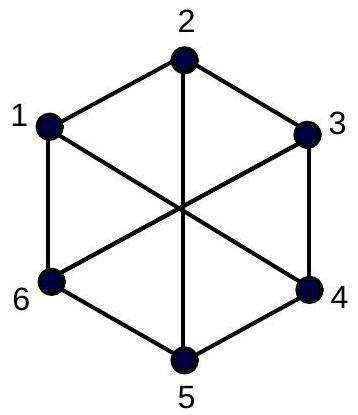
\includegraphics[max width=\textwidth, center]{2025_09_05_76a00afb34b0e185ce5bg-14}

Tomemos como $S$ al conjunto de vértices del hexágono, es decir, $S=\{1,2,3,4,5,6\}$ y definamos bloques de 2 elementos en la forma: $x y$ es un bloque si y sólo si hay una línea recta que une $x$ con $y$. Luego los bloques son

$$
12,23,34,45,56,16,14,25 \text { y } 36
$$

Como en cada vértice inciden exactamente 3 líneas, ahora se tiene que\\
i) $S$ tiene 6 elementos\\
ii) Cada bloque tiene 2 elementos\\
iii) Cada subconjunto de cardinal 1 de $S$ está contenido en exactamente 3 bloques

Definición: Un diseño de parámetros $t-(\nu, k, \lambda)$ es un par ordenado ( $S, C$ ) de conjuntos que satisface\\
i) $S$ tiene $\nu$ elementos\\
ii) Cada elemento de $C$ es un subconjunto de $S$ de cardinal $k$\\
iii) Todo subconjunto de $S$ de cardinal $t$ está contenido en exactamente $\lambda$ elementos de $C$

Llamaremos bloques a los elementos de $C$ y puntos a los elementos de $S$. Diremos que un diseño de parámetros $t-(\nu, k, \lambda)$ es no trivial si $1<t<k<\nu$ y no todo subconjunto de $S$ de cardinal $k$ es un bloque.

Dados $t, \nu, k$ y $\lambda$ no siempre existe un diseño de parámetros $t-(\nu, k, \lambda)$. En general, determinar si existe es un problema difícil.

En el ejemplo 1 hemos construído un diseño de parámetros $2-(7,3,1)$, en el ejemplo 2 un diseño de parámetros $2-(7,4,2)$, en el ejemplo 3 un diseño de parámetros $3-(16,4,1)$ y en el ejemplo 4 un diseño de parámetros 1-( $6,2,3$ ).

Matriz de incidencia. Sea ( $S, C$ ) un diseño de parámetros $t-(\nu, k, \lambda)$. Si fijamos un orden para los elementos de $S$ y fijamos un orden para los bloques, entonces podemos representar el diseño utilizando una matriz, llamada la matriz de incidencia del diseño. Esta es una matriz $D=\left\|d_{i j}\right\|$ de ceros y unos que tiene una fila por cada bloque y una columna por cada punto y que se define en la forma:

$$
d_{i j}= \begin{cases}1 & \text { si el } j \text {-ésimo elemento de } S \text { está en el } i \text {-ésimo bloque } \\ 0 & \text { si no }\end{cases}
$$

Notar que cada fila de esta matriz contiene exactamente $k$ unos ya que cada bloque tiene cardinal $k$.\\
Por ejemplo, la matriz de incidencia del diseño del ejemplo 4 es

$$
\left(\begin{array}{llllll}
1 & 1 & 0 & 0 & 0 & 0 \\
0 & 1 & 1 & 0 & 0 & 0 \\
0 & 0 & 1 & 1 & 0 & 0 \\
0 & 0 & 0 & 1 & 1 & 0 \\
0 & 0 & 0 & 0 & 1 & 1 \\
1 & 0 & 0 & 0 & 0 & 1 \\
1 & 0 & 0 & 1 & 0 & 0 \\
0 & 1 & 0 & 0 & 1 & 0 \\
0 & 0 & 1 & 0 & 0 & 1
\end{array}\right)
$$

Definición: Un diseño cuadrado de parámetros ( $\nu, k, \lambda$ ) es un par ordenado ( $S, C$ ) de conjuntos que satisface\\
i) $S$ y $C$ son conjuntos de cardinal $\nu$\\
ii) Cada elemento de $C$ es un subconjunto de $S$ de cardinal $k$\\
iii) Todo subconjunto de $S$ de cardinal 2 está contenido en exactamente $\lambda$ elementos de $C$ iv) Todo subconjunto de $S$ de cardinal 1 está contenido en exactamente $k$ elementos de $C$ v) $2<k<\nu$ y no todo subconjunto de $S$ de cardinal $k$ es un bloque

Es decir, un diseño cuadrado ( $S, C$ ) de parámetros ( $\nu, k, \lambda$ ) es un diseño no trivial de parámetros $2-(\nu, k, \lambda)$ que tiene $\nu$ bloques y tal que todo punto de $S$ pertenece a exactamente $k$ bloques.\\
Dejamos como tarea al lector verificar que los diseños de los ejemplos 1 y 2 son diseños cuadrados de parámetros $(7,3,1)$ y $(7,4,2)$ respectivamente y sus matrices de incidencia son

$$
\left(\begin{array}{lllllll}
0 & 1 & 0 & 1 & 0 & 1 & 0 \\
1 & 0 & 0 & 0 & 0 & 1 & 1 \\
1 & 0 & 0 & 1 & 1 & 0 & 0 \\
0 & 1 & 0 & 0 & 1 & 0 & 1 \\
1 & 1 & 1 & 0 & 0 & 0 & 0 \\
0 & 0 & 1 & 1 & 0 & 0 & 1 \\
0 & 0 & 1 & 0 & 1 & 1 & 0
\end{array}\right) \quad \text { y } \quad\left(\begin{array}{lllllll}
1 & 0 & 1 & 0 & 1 & 0 & 1 \\
0 & 1 & 1 & 1 & 1 & 0 & 0 \\
0 & 1 & 1 & 0 & 0 & 1 & 1 \\
1 & 0 & 1 & 1 & 0 & 1 & 0 \\
0 & 0 & 0 & 1 & 1 & 1 & 1 \\
1 & 1 & 0 & 0 & 1 & 1 & 0 \\
1 & 1 & 0 & 1 & 0 & 0 & 1
\end{array}\right)
$$

Notar que la matriz de incidencia de un diseño cuadrado es una matriz cuadrada de ceros y unos. Más aún, la condición i) de la definición es equivalente a que $D$ sea una matriz de $\nu \times \nu$, ii) es equivalente a que cada fila de $D$ contenga exactamente $k$ unos, iii) es equivalente a que el producto escalar de dos columnas distintas de $D$ sea igual a $\lambda$, iv) es equivalente a que cada columna de $D$ contenga exactamente $k$ unos y v) es equivalente a pedir $2<k<\nu-1$.\\
Las condiciones iii) y iv) son equivalentes a que el producto escalar de las columnas $i$ y $j$ de $D$ sea igual a $\lambda$ si $i \neq j$ y a $k$ si $i=j$. Luego, si $D$ es la matriz de incidencia de un diseño cuadrado de parámetros ( $\nu, k, \lambda$ ) entonces

$$
D^{t} . D=\left(\begin{array}{cccccc}
k & \lambda & \lambda & \ldots & \lambda & \lambda \\
\lambda & k & \lambda & \ldots & \lambda & \lambda \\
\vdots & \vdots & \vdots & & \vdots & \vdots \\
\lambda & \lambda & \lambda & \ldots & k & \lambda \\
\lambda & \lambda & \lambda & \ldots & \lambda & k
\end{array}\right)
$$

Veamos ahora que $D \cdot D^{t}=D^{t} \cdot D$, lo que implica que el producto escalar de dos filas distintas de $D$ es igual a $\lambda$.\\
Sean $I$ la matriz identidad de orden $\nu$ y sea $J$ la matriz de $\nu$ filas y $\nu$ columnas que tiene todos sus coeficientes iguales a 1 . Entonces $D^{t} . D=\lambda J+(k-\lambda) I$. Además, $D . J=k J$ por ii) y $J . D=k J$ por iv).\\
Como $J . D=D . J$ y por el ejercicio 10 de la práctica $5 D$ es inversible, entonces se tiene que $J=D . J . D^{-1}$. Luego,

$$
\begin{aligned}
D \cdot D^{t} & =D \cdot D^{t} \cdot D \cdot D^{-1}=D[\lambda J+(k-\lambda) I] D^{-1}= \\
& =\lambda D \cdot J \cdot D^{-1}+(k-\lambda) I=\lambda J+(k-\lambda) I
\end{aligned}
$$

Recíprocamente, si $D$ es una matriz de $\nu \times \nu$ con coeficientes ceros y unos que satisface $D^{t} . D=\lambda J+(k-\lambda) I$ y $D . J=k J=J . D$ entonces $D$ es la matriz de incidencia de un diseño cuadrado de parámetros $(\nu, k, \lambda)$.

Ejemplo 5. Si $p$ es un primo congruente a 3 módulo 4, podemos construír un diseño cuadrado de parámetros ( $p, \frac{p+1}{2}, \frac{p+1}{4}$ ) utilizando los residuos cuadráticos módulo $p$. Veamos cómo hacer esto en el caso $p=11$.\\
Primero construímos el conjunto de todos los residuos cuadráticos módulo $p$,

$$
Q=\left\{r_{p}\left(x^{2}\right) / x=0,1,2, \ldots, p-1\right\}
$$

Ahora consideremos el vector $u=\left(u_{0}, u_{1}, \ldots, u_{p-1}\right)$ definido por

$$
u_{j}= \begin{cases}1 & \text { si } j \in Q \\ 0 & \text { si no }\end{cases}
$$

y construyamos una matriz $D$ de ceros y unos que tiene $p$ filas y $p$ columnas cuyas filas son las permutaciones cíclicas de $u$ :

$$
D=\left(\begin{array}{cccccc}
u_{0} & u_{1} & u_{2} & \ldots & u_{p-2} & u_{p-1} \\
u_{p-1} & u_{0} & u_{1} & \ldots & u_{p-3} & u_{p-2} \\
u_{p-2} & u_{p-1} & u_{0} & \ldots & u_{p-4} & u_{p-3} \\
\vdots & \vdots & \vdots & & \vdots & \vdots \\
u_{1} & u_{2} & u_{3} & \ldots & u_{p-1} & u_{0}
\end{array}\right)
$$

En nuestro caso, $Q=\{0,1,3,4,5,9\}, u=(1,1,0,1,1,1,0,0,0,1,0) y$

$$
D=\left(\begin{array}{lllllllllll}
1 & 1 & 0 & 1 & 1 & 1 & 0 & 0 & 0 & 1 & 0 \\
0 & 1 & 1 & 0 & 1 & 1 & 1 & 0 & 0 & 0 & 1 \\
1 & 0 & 1 & 1 & 0 & 1 & 1 & 1 & 0 & 0 & 0 \\
0 & 1 & 0 & 1 & 1 & 0 & 1 & 1 & 1 & 0 & 0 \\
0 & 0 & 1 & 0 & 1 & 1 & 0 & 1 & 1 & 1 & 0 \\
0 & 0 & 0 & 1 & 0 & 1 & 1 & 0 & 1 & 1 & 1 \\
1 & 0 & 0 & 0 & 1 & 0 & 1 & 1 & 0 & 1 & 1 \\
1 & 1 & 0 & 0 & 0 & 1 & 0 & 1 & 1 & 0 & 1 \\
1 & 1 & 1 & 0 & 0 & 0 & 1 & 0 & 1 & 1 & 0 \\
0 & 1 & 1 & 1 & 0 & 0 & 0 & 1 & 0 & 1 & 1 \\
1 & 0 & 1 & 1 & 1 & 0 & 0 & 0 & 1 & 0 & 1
\end{array}\right)
$$

Ahora tomamos $S=\{0,1,2,3, \ldots, p-1\}$ y los $p$ bloques definidos por: el $j$-ésimo elemento de $S$ está en el $i$-ésimo bloque si y sólo si $d_{i j}=1$.\\
En nuestro caso $S=\{0,1,2,3,4,5,6,7,8,9,10\}$ y los 11 bloques son

$$
\begin{array}{llll}
\{0,1,3,4,5,9\}, & \{1,2,4,5,6,10\}, & \{0,2,3,5,6,7\}, & \{1,3,4,6,7,8\}, \\
\{2,4,5,7,8,9\}, & \{3,5,6,8,9,10\}, & \{0,4,6,7,9,10\}, & \{0,1,5,7,8,10\}, \\
\{0,1,2,6,8,9\}, & \{1,2,3,7,9,10\}, & \{0,2,3,4,8,10\} &
\end{array}
$$

El lector puede verificar que este es un diseño cuadrado de parámetros ( $11,6,3$ ) cuya matriz de incidencia es $D$. En el caso general, para demostrar que con esta construcción se obtiene un diseño cuadrado de parámetros ( $p, \frac{p+1}{2}, \frac{p+1}{4}$ ) se utiliza el símbolo de Legendre. Esta demostración puede hallarse en\\
M. J. Erickson, Introduction to Combinatorics

Ejemplo 6. Si ahora cambiamos cada 1 de $D$ por un 0 y cada 0 por un 1 obtenemos la matriz

$$
D^{\prime}=\left(\begin{array}{lllllllllll}
0 & 0 & 1 & 0 & 0 & 0 & 1 & 1 & 1 & 0 & 1 \\
1 & 0 & 0 & 1 & 0 & 0 & 0 & 1 & 1 & 1 & 0 \\
0 & 1 & 0 & 0 & 1 & 0 & 0 & 0 & 1 & 1 & 1 \\
1 & 0 & 1 & 0 & 0 & 1 & 0 & 0 & 0 & 1 & 1 \\
1 & 1 & 0 & 1 & 0 & 0 & 1 & 0 & 0 & 0 & 1 \\
1 & 1 & 1 & 0 & 1 & 0 & 0 & 1 & 0 & 0 & 0 \\
0 & 1 & 1 & 1 & 0 & 1 & 0 & 0 & 1 & 0 & 0 \\
0 & 0 & 1 & 1 & 1 & 0 & 1 & 0 & 0 & 1 & 0 \\
0 & 0 & 0 & 1 & 1 & 1 & 0 & 1 & 0 & 0 & 1 \\
1 & 0 & 0 & 0 & 1 & 1 & 1 & 0 & 1 & 0 & 0 \\
0 & 1 & 0 & 0 & 0 & 1 & 1 & 1 & 0 & 1 & 0
\end{array}\right)
$$

$D^{\prime}$ es la matriz de incidencia de un diseño cuadrado de parámetros ( $11,5,2$ ) (ver ejercicio 11 de la práctica 5).

Ejemplo 7. Considremos la sucesión de matrices definida por

$$
H_{0}=\left(\begin{array}{cc}
1 & 1 \\
-1 & 1
\end{array}\right) \quad H_{m+1}=\left(\begin{array}{cc}
H_{m} & H_{m} \\
-H_{m} & H_{m}
\end{array}\right)
$$

Por ejemplo,

$$
H_{1}=\left(\begin{array}{cccc}
1 & 1 & 1 & 1 \\
-1 & 1 & -1 & 1 \\
-1 & -1 & 1 & 1 \\
1 & -1 & -1 & 1
\end{array}\right) \quad y \quad H_{2}=\left(\begin{array}{cccccccc}
1 & 1 & 1 & 1 & 1 & 1 & 1 & 1 \\
-1 & 1 & -1 & 1 & -1 & 1 & -1 & 1 \\
-1 & -1 & 1 & 1 & -1 & -1 & 1 & 1 \\
1 & -1 & -1 & 1 & 1 & -1 & -1 & 1 \\
-1 & -1 & -1 & -1 & 1 & 1 & 1 & 1 \\
1 & -1 & 1 & -1 & -1 & 1 & -1 & 1 \\
1 & 1 & -1 & -1 & -1 & -1 & 1 & 1 \\
-1 & 1 & 1 & -1 & 1 & -1 & -1 & 1
\end{array}\right)
$$

$H_{m}$ tiene $2^{m+1}$ filas y $2^{m+1}$ columnas y satisface $H_{m}^{t} \cdot H_{m}=H_{m} \cdot H_{m}^{t}=2^{m+1} I$, donde $I$ denota la matriz identidad.\\
Sea $m \geq 2$. Si eliminamos la primera fila y la última columna de $H_{m}$ y luego cambiamos cada -1 por 0 obtenemos la matriz de incidencia de un diseño cuadrado de parámetros $\left(2^{m+1}-1,2^{m}-1,2^{m-1}-1\right)$.

En efecto, si $X$ la matriz que resulta de eliminar la primera fila y la última columna de $H_{m}$ es claro que $X . J=J . X=-J$ y por lo tanto $X^{t} . J=J . X^{t}=-J$, donde $J$ dentota la matriz que tiene todos sus coeficientes iguales a 1 . Además, como $H_{m}^{t} \cdot H_{m}=H_{m} \cdot H_{m}^{t}=2^{m+1} I$ entonces resulta que $X^{t} . X=X . X^{t}=2^{m+1} I-J$.\\
Si ahora cambiamos cada -1 por un 0 la matriz resultante es $D=\frac{1}{2}(X+J)$, Luego, tomando $\nu=2^{m+1}-1, \lambda=2^{m-1}-1$ y $k=2^{m}-1$ resulta que $D$ es una matriz de $\nu \times \nu$ con coeficientes ceros y unos y valen

$$
\begin{aligned}
D . J & =\frac{1}{2}(X+J) J=\frac{1}{2}\left(X . J+J^{2}\right)=\frac{1}{2}\left(-J+\left(2^{m+1}-1\right) J\right)=\left(2^{m}-1\right) J=k J \\
J . D & =\frac{1}{2} J(X+J)=\frac{1}{2}\left(J . X+J^{2}\right)=\frac{1}{2}\left(-J+\left(2^{m+1}-1\right) J\right)=\left(2^{m}-1\right) J=k J \\
D^{t} . D & =\frac{1}{4}\left(X^{t}+J^{t}\right)(X+J)=\frac{1}{4}\left(X^{t}+J\right)(X+J)= \\
& =\frac{1}{4}\left(X^{t} . X+X . J+J . X^{t}+J^{2}\right)=\frac{1}{4}\left(2^{m+1} I-J-J-J+\left(2^{m+1}-1\right) J\right)= \\
& =2^{m-1} I+\left(2^{m-1}-1\right) J=(k-\lambda) I+\lambda J
\end{aligned}
$$

Por lo tanto hemos probado que $D$ es la matriz de incidencia de un diseño cuadrado de parámetros $(\nu, k, \lambda)=\left(2^{m+1}-1,2^{m}-1,2^{m-1}-1\right)$.

\section*{4. Códigos y diseños.}
Al comienzo de la sección 3., utilizando un código que corrige un error, construímos un diseño cuadrado de parámetros ( $7,3,1$ ) (ejemplo 1) y luego, tomando el complemento de sus bloques, obtuvimos un diseño cuadrado de parámetros ( $7,4,2$ ) (ejemplo 2). Ahora, utilizando el diseño cuadrado de parámetros $(11,6,3)$ y su complemento que construímos en la sección anterior (ejemplos 5 y 6), obtendremos un código que corrige 2 errores.\\
Sea $A \subseteq F^{11}$ el código formado por las filas de las matrices $D$ y $D^{\prime}$ correspondientes a cada uno de los mencionados diseños y las palabras 11111111111 y 00000000000 . Veamos que $d(A)=5$.\\
Dado un vector binario $u$ de longitud $n$, denotemos por $w(u)$ a la cantidad de unos que contiene $u$. Usando el ejercicio 4 de la práctica 5 resulta que $d(u, v)=w(u)+w(v)-2 u . v$, donde $u . v$ es el producto escalar de $u$ y $v$ (considerados como vectores de coordenadas reales).\\
Como $D$ y $D^{\prime}$ son las matrices de incidencia de diseños cuadrados de parámetros ( $11,6,3$ ) y ( $11,5,2$ ) respectivamente entonces cada fila de $D$ contiene exactamente 6 unos, cada fila de $D^{\prime}$ contiene exactamente 5 unos, el producto escalar de dos filas distintas de $D$ es igual a 3 y el producto escalar de dos filas distintas de $D^{\prime}$ es igual a 2 .\\
Dado un vector binario $v$ denotaremos por $\bar{v}$ al complemento de $v$, es decir, al vector que se obtiene cambiando cada 1 de $v$ por un 0 y cada 0 por un 1 .

Sean $u, v \in A$, con $u \neq v$. Si $u$ y $v$ son dos filas de $D$ entonces $d(u, v)=6+6-2.3=6$, si $u$ y $v$ son dos filas de $D^{\prime}$ entonces $d(u, v)=5+5-2.2=6$, si $u$ es una fila de $D$ y $v$ es una fila de $D^{\prime}$ entonces el complemento $\bar{v}$ de $v$ es una fila de $D$ y por lo tanto, usando el ejercicio 5 de la práctica 5 resulta que

$$
d(u, v)=11-d(u, \bar{v})= \begin{cases}11-6=5 & \text { si } u \neq \bar{v} \\ 11-0=11 & \text { si } u=\bar{v}\end{cases}
$$

Finalmente, si $u=11111111111$ entonces $d(u, v)$ es igual la cantidad de ceros de $v$ de donde

$$
d(u, v)= \begin{cases}5 & \text { si } v \text { es una fila de } D \\ 6 & \text { si } v \text { es una fila de } D^{\prime} \\ 11 & \text { si } v=00000000000\end{cases}
$$

y si $u=00000000000$ entonces $d(u, v)$ es igual a la cantidad de unos de $v$ de donde

$$
d(u, v)= \begin{cases}6 & \text { si } v \text { es una fila de } D \\ 5 & \text { si } v \text { es una fila de } D^{\prime} \\ 11 & \text { si } v=11111111111\end{cases}
$$

Hemos probado entonces que $d(A)=5$, Luego, este es un código de 24 palabras que corrige 2 errores.

En general, si $D$ es la matriz de incidencia de un diseño cuadrado de parámetros ( $\nu, k, \lambda$ ) y $D^{\prime}$ es la matriz de incidencia de su complemento, que tiene parámetros ( $\nu, \nu-k, \nu-2 k+\lambda$ ). Como $2(\nu-k)-2(\nu-2 k+\lambda)=2(k-\lambda)$, entonces el código $A \subseteq F^{\nu}$ formado por las filas de $D$, las de $D^{\prime}$ y las palabras $111 \ldots 1$ y $000 \ldots 0$ tiene $2 \nu+2$ palabras y satisface:\\
Si $u, v \in A, u \neq v$,

$$
d(u, v)= \begin{cases}2(k-\lambda) & \text { si } u \text { y } v \text { son filas de } D \text { o } u \text { y } v \text { son filas de } D^{\prime} \\ \nu-2(k-\lambda) & \text { si } u \text { es una fila de } D, v \text { es una fila de } D^{\prime} \text { y } u \neq \bar{v} \\ \nu & \text { si } u \text { es una fila de } D, v \text { es una fila de } D^{\prime} \text { y } u=\bar{v} \\ \nu-k & \text { si } u=111 \ldots 1 \text { y } v \text { es una fila de } D \\ k & \text { si } u=111 \ldots 1 \text { y } v \text { es una fila de } D^{\prime} \\ \nu-k & \text { si } u=000 \ldots 0 \text { y } v \text { es una fila de } D^{\prime} \\ k & \text { si } u=000 \ldots 0 \text { y } v \text { es una fila de } D \\ \nu & \text { si } u=111 \ldots 1 \text { y } v=000 \ldots 0\end{cases}
$$

Aplicando esto al diseño cuadrado de parámetros $(\nu, k, \lambda)=\left(2^{m+1}-1,2^{m}-1,2^{m-1}-1\right)$, ( $m \geq 2$ ), que construímos en el ejemplo 7 obtenemos un código $A \subseteq F^{2^{m+1}-1}$ que tiene $2^{m+2}$ palabras. Además, como $2(k-\lambda)=2^{m}, \nu-2(k-\lambda)=2^{m}-1, \nu=2^{m+1}-1$, $k=2^{m}-1$ y $\nu-k=2^{m}$ entonces $d(A)=2^{m}-1$. Luego, este es un código que corrige $2^{m-1}-1$ errores.

Finalmente, veamos cómo podemos construír, nuevamente utilizando el diseño cuadrado de parámetros ( $11,6,3$ ), el código de Golay $A \subseteq F^{23}$ que satisface $|A|=2^{12}$ y $d(A) \geq 7$. Este es un código perfecto que corrige 3 errores.

Sea $D$ la matriz de incidencia del el diseño cuadrado de parámetros $(11,6,3)$ y sea $G$ la matriz de 12 filas y 24 columnas\\
donde $I_{11}$ es la matriz identidad de orden 11. Luego $G$ es la matriz

$$
\left(\begin{array}{llllllllllllllllllllllll}
1 & 1 & 0 & 0 & 0 & 0 & 0 & 0 & 0 & 0 & 0 & 0 & 0 & 1 & 1 & 0 & 1 & 1 & 1 & 0 & 0 & 0 & 1 & 0 \\
1 & 0 & 1 & 0 & 0 & 0 & 0 & 0 & 0 & 0 & 0 & 0 & 0 & 0 & 1 & 1 & 0 & 1 & 1 & 1 & 0 & 0 & 0 & 1 \\
1 & 0 & 0 & 1 & 0 & 0 & 0 & 0 & 0 & 0 & 0 & 0 & 0 & 1 & 0 & 1 & 1 & 0 & 1 & 1 & 1 & 0 & 0 & 0 \\
1 & 0 & 0 & 0 & 1 & 0 & 0 & 0 & 0 & 0 & 0 & 0 & 0 & 0 & 1 & 0 & 1 & 1 & 0 & 1 & 1 & 1 & 0 & 0 \\
1 & 0 & 0 & 0 & 0 & 1 & 0 & 0 & 0 & 0 & 0 & 0 & 0 & 0 & 0 & 1 & 0 & 1 & 1 & 0 & 1 & 1 & 1 & 0 \\
1 & 0 & 0 & 0 & 0 & 0 & 1 & 0 & 0 & 0 & 0 & 0 & 0 & 0 & 0 & 0 & 1 & 0 & 1 & 1 & 0 & 1 & 1 & 1 \\
1 & 0 & 0 & 0 & 0 & 0 & 0 & 1 & 0 & 0 & 0 & 0 & 0 & 1 & 0 & 0 & 0 & 1 & 0 & 1 & 1 & 0 & 1 & 1 \\
1 & 0 & 0 & 0 & 0 & 0 & 0 & 0 & 1 & 0 & 0 & 0 & 0 & 1 & 1 & 0 & 0 & 0 & 1 & 0 & 1 & 1 & 0 & 1 \\
1 & 0 & 0 & 0 & 0 & 0 & 0 & 0 & 0 & 1 & 0 & 0 & 0 & 1 & 1 & 1 & 0 & 0 & 0 & 1 & 0 & 1 & 1 & 0 \\
1 & 0 & 0 & 0 & 0 & 0 & 0 & 0 & 0 & 0 & 1 & 0 & 0 & 0 & 1 & 1 & 1 & 0 & 0 & 0 & 1 & 0 & 1 & 1 \\
1 & 0 & 0 & 0 & 0 & 0 & 0 & 0 & 0 & 0 & 0 & 1 & 0 & 1 & 0 & 1 & 1 & 1 & 0 & 0 & 0 & 1 & 0 & 1 \\
0 & 0 & 0 & 0 & 0 & 0 & 0 & 0 & 0 & 0 & 0 & 0 & 1 & 1 & 1 & 1 & 1 & 1 & 1 & 1 & 1 & 1 & 1 & 1
\end{array}\right)
$$

Ahora consideremos la transformación lineal $g: \mathbb{Z}_{2}^{12} \longrightarrow \mathbb{Z}_{2}^{24}$ definida por $g(u)=u . G$. Como las columnas $2,3, \ldots, 13$ de $G$ son linealmente independientes entonces $\operatorname{rg}(G)=12$. Luego, $B=\operatorname{Im}(g)=\left\{u \cdot G / u \in \mathbb{Z}^{12}\right\}$ es un $\mathbb{Z}_{2}$-espacio vectorial de dimensión 12 y por lo tanto $|B|=2^{12}$. Además, como $B$ es el subespacio de $\mathbb{Z}_{2}^{24}$ generado por las filas de $G$ y como los escalares son 0 o 1 entonces todo elemento no nulo de $B$ es suma de filas de $G$. Probaremos que la distancia de Hamming entre dos elementos distintos de $B$ es mayor o igual que 8. Luego, si $A$ es el código que se obtiene eliminando la primera coordenada de cada elemento de $B$ resulta que $A \subseteq F^{23},|A|=2^{12}$ y $d(A) \geq 7$.\\
Por el ejercicio 4 ii), si $u$ y $v$ son dos elementos distintos de $B$ entonces $d(u, v)=w(u+v)$ (suma hecha en $\mathbb{Z}_{2}^{24}$ ). Luego, lo que debemos probar es que $w(u+v) \geq 8 \mathrm{y}$, para ello, basta probar que $w(x) \geq 8$ para todo $x$ no nulo de $B$, ya que $u+v \in B$ pues $B$ es un subespacio de $\mathbb{Z}_{2}^{24}$ y $u+v \neq 0$ pues $u \neq v$.

Queremos probar que $w(x) \geq 8$ para todo $x$ no nulo de $B$. Para ello usaremos que si $a, b \in \mathbb{Z}_{2}^{24}$ entonces $w(a+b)=w(a)+w(b)-2 a . b$, donde $a+b$ es la suma en $\mathbb{Z}_{2}^{24}$ y $a . b$ es el producto escalar de $a$ y $b$ (ejercicio 4.) y que el producto escalar de dos filas de $G$ es siempre par (esto puede verificarse haciendo todos los posibles productos).

Afirmación: Para todo $r \geq 1$ vale: Si $a$ es suma de $r$ filas de $G$ entonces $w(a)$ es un múltiplo de 4 .

Demostración: Por inducción en $r$. Si $r=1$ entonces $a$ es una fila de $G$. En este caso $w(a)=8$ о $w(a)=12$.\\
Supongamos ahora que vale para $r$ y supongamos que $a$ es suma de $r+1$ filas de $G$

$$
a=F_{i_{1}}+F_{i_{2}}+\cdots+F_{i_{r}}+F_{i_{r+1}}
$$

\section*{Entonces}
$$
\begin{aligned}
w(a) & =w\left(F_{i_{1}}+F_{i_{2}}+\cdots+F_{i_{r}}\right)+w\left(F_{i_{r+1}}\right)-2\left(F_{i_{1}}+F_{i_{2}}+\cdots+F_{i_{r}}\right) \cdot F_{i_{r+1}}= \\
& =w\left(F_{i_{1}}+F_{i_{2}}+\cdots+F_{i_{r}}\right)+w\left(F_{i_{r+1}}\right)-2 F_{i_{1}} \cdot F_{i_{r+1}}-2 F_{i_{2}} \cdot F_{i_{r+1}}-\cdots-2 F_{i_{r}} \cdot F_{i_{r+1}}
\end{aligned}
$$

Como $w\left(F_{i_{1}}+F_{i_{2}}+\cdots+F_{i_{r}}\right)$ es múltiplo de 4 por hipótesis inductiva, $w\left(F_{i_{r+1}}\right)=8$ o 12 y cada producto escalar es par, resulta que $w(a)$ es múltiplo de 4 .\\
Luego, $w(x)$ es múltiplo de 4 para todo $x \in B$ ya que todo elemento de $B$ es suma de filas de $G$. Por lo tanto, los posibles valores de $w(x)$ para $x \in B$ son $0,4,8,12,16,20$ y 24 . Como $w(x)=0$ sii $x=0$, sólo nos falta probar que $w(x) \neq 4$ para todo $x$ no nulo de $B$. Sea $L(G)$ la matriz formada por las primeras 12 columnas de $G$

$$
L(G)=\left(\begin{array}{cccccccccccc}
1 & 1 & 0 & 0 & 0 & 0 & 0 & 0 & 0 & 0 & 0 & 0 \\
1 & 0 & 1 & 0 & 0 & 0 & 0 & 0 & 0 & 0 & 0 & 0 \\
1 & 0 & 0 & 1 & 0 & 0 & 0 & 0 & 0 & 0 & 0 & 0 \\
1 & 0 & 0 & 0 & 1 & 0 & 0 & 0 & 0 & 0 & 0 & 0 \\
1 & 0 & 0 & 0 & 0 & 1 & 0 & 0 & 0 & 0 & 0 & 0 \\
1 & 0 & 0 & 0 & 0 & 0 & 1 & 0 & 0 & 0 & 0 & 0 \\
1 & 0 & 0 & 0 & 0 & 0 & 0 & 1 & 0 & 0 & 0 & 0 \\
1 & 0 & 0 & 0 & 0 & 0 & 0 & 0 & 1 & 0 & 0 & 0 \\
1 & 0 & 0 & 0 & 0 & 0 & 0 & 0 & 0 & 1 & 0 & 0 \\
1 & 0 & 0 & 0 & 0 & 0 & 0 & 0 & 0 & 0 & 1 & 0 \\
1 & 0 & 0 & 0 & 0 & 0 & 0 & 0 & 0 & 0 & 0 & 1 \\
0 & 0 & 0 & 0 & 0 & 0 & 0 & 0 & 0 & 0 & 0 & 0
\end{array}\right)
$$

sea $R(G)$ la matriz formada por las últimas 12 columnas de $G$

$$
R(G)=\left(\begin{array}{llllllllllll}
0 & 1 & 1 & 0 & 1 & 1 & 1 & 0 & 0 & 0 & 1 & 0 \\
0 & 0 & 1 & 1 & 0 & 1 & 1 & 1 & 0 & 0 & 0 & 1 \\
0 & 1 & 0 & 1 & 1 & 0 & 1 & 1 & 1 & 0 & 0 & 0 \\
0 & 0 & 1 & 0 & 1 & 1 & 0 & 1 & 1 & 1 & 0 & 0 \\
0 & 0 & 0 & 1 & 0 & 1 & 1 & 0 & 1 & 1 & 1 & 0 \\
0 & 0 & 0 & 0 & 1 & 0 & 1 & 1 & 0 & 1 & 1 & 1 \\
0 & 1 & 0 & 0 & 0 & 1 & 0 & 1 & 1 & 0 & 1 & 1 \\
0 & 1 & 1 & 0 & 0 & 0 & 1 & 0 & 1 & 1 & 0 & 1 \\
0 & 1 & 1 & 1 & 0 & 0 & 0 & 1 & 0 & 1 & 1 & 0 \\
0 & 0 & 1 & 1 & 1 & 0 & 0 & 0 & 1 & 0 & 1 & 1 \\
0 & 1 & 0 & 1 & 1 & 1 & 0 & 0 & 0 & 1 & 0 & 1 \\
1 & 1 & 1 & 1 & 1 & 1 & 1 & 1 & 1 & 1 & 1 & 1
\end{array}\right)
$$

y, para cada $x \in B$ denotemos por $L(x)$ y $R(x)$ a los vectores de $\mathbb{Z}_{2}^{12}$ formados por las primeras 12 y las últimas 12 coordenadas de $x$ respectivamente.

Sea $x$ un vector no nulo de $B$. Como $x$ es suma de filas de $G$ entonces $L(x)$ es suma de filas de $L(G)$. Usando esto es fácil ver que si $x$ es suma de $r$ filas de $G$ entonces

\[
w(L(x))= \begin{cases}r & \text { si } r \text { es par }  \tag{1}\\ r+1 & \text { si } r \text { es impar y ninguna de las filas es la fila } 12 \\ r-1 & \text { si } r \text { es impar y una de las filas es la fila } 12\end{cases}
\]

En particular, $w(L(x))$ es par. Supongamos ahora que $w(x)=4$. Entonces los únicos casos posibles son:

\begin{enumerate}
  \item $w(L(x))=0$ y $w(R(x))=4$
  \item $w(L(x))=2$ y $w(R(x))=2$
  \item $w(L(x))=4$ y $w(R(x))=0$
\end{enumerate}

Veamos que ninguno de estos casos puede ocurrir.\\
Caso 1. $w(L(x))=0$ y $w(R(x))=4$\\
Si $w(L(x))=0$ entonces de (1) resulta que $r=1$ y una de las filas es la fila 12. Luego, $x$ es la fila 12. Pero entonces $w(R(x))=12 \neq 4$.\\
Caso 2. $w(L(x))=2$ y $w(R(x))=2$\\
Si $w(L(x))=2$ entonces de (1) resulta que $r=2$ o bien $r=1$ y ninguna de las filas es la fila 12 o bien $r=3$ y una de las filas es la fila 12.\\
Luego, $x$ es suma de dos filas de $G$ o $x$ es una fila distinta de la fila 12 o $x$ es la fila 12 más otras dos filas de $G$ y por lo tanto $R(x)$ es suma de dos filas de $R(G)$ o $R(x)$ es una fila de $R(G)$ distinta de la fila 12 o $R(x)$ es la fila 12 más otras dos filas de $R(G)$. El lector puede verificar que en todos estos casos resulta que $w(R(x))=6 \neq 4$.\\
Caso 3. $w(L(x))=4$ y $w(R(x))=0$\\
Como $x \in B$ entonces $x=u . G$ para algún $u=\left(u_{1}, u_{2}, \ldots, u_{12}\right) \in \mathbb{Z}_{2}^{12}$.

Luego,

$$
x=u_{1} F_{1}+u_{2} F_{2}+\cdots+u_{12} F_{12}
$$

donde $F_{i}$ denota la $i$-ésima fila de $G$. Entonces, como $w(R(x))=0$ se tiene que

$$
\begin{aligned}
(0,0,0,0,0,0,0,0,0,0,0,0) & =R(x)=u_{1} R\left(F_{1}\right)+u_{2} R\left(F_{2}\right)+\cdots+u_{12} R\left(F_{12}\right)= \\
& =\left(u_{1}, u_{2}, \ldots, u_{12}\right) \cdot R(G)=u \cdot R(G)
\end{aligned}
$$

Esto significa que $u \in N u(f)$, donde $f: \mathbb{Z}_{2}^{12} \longrightarrow \mathbb{Z}_{2}^{12}$ es la transformación lineal definida por $f(y)=y \cdot R(G)$. Además, siendo $x$ no nulo resulta que $u$ no es el vector nulo.\\
Como $\operatorname{rg}(R(G))=11$ entonces $N u(f)$ es un espacio vectorial de dimensión 1 sobre $\mathbb{Z}_{2}$ y por lo tanto tiene cardinal 2.

Luego, $u$ debe ser el único vector no nulo de $N u(f)$. Observando que la suma de las primeras once filas de $R(G)$ es cero se tiene que $(1,1,1,1,1,1,1,1,1,1,1,0) \in N u(f)$. Luego, $u=(1,1,1,1,1,1,1,1,1,1,1,0)$ de donde resulta que $x=u \cdot G=F_{1}+F_{2}+\cdots+F_{11}$ Pero entonces $L(x)=(1,1,1,1,1,1,1,1,1,1,1,1)$ y por lo tanto $w(L(X))=12 \neq 4$.

\section*{5. Cuadrados latinos.}
Supongamos que queremos comparar el rendimiento de $n$ variedades de trigo. Si plantamos cada variedad en una franja del terreno podría ocurrir que el trigo plantado en la primera franja tuviera un alto rendimiento debido a que esa zona del terreno es más fértil que las otras y no porque esa variedad de trigo sea en realidad la de mayor rendimiento. Para evitar que las diferencias en la fertilidad del suelo influyan en los resultados de nuestro experimento, conviene dividir el terreno en $n^{2}$ parcelas y plantar cada una de las $n$ variedades de trigo en $n$ parcelas de manera que cada franja (horizontal o vertical) del terreno contenga las $n$ variedades. Por ejemplo, para $n=3$, las variedades $a, b$ y $c$ podrían disponerse en la forma

\begin{center}
\begin{tabular}{|c|c|c|}
\hline
$a$ & $b$ & $c$ \\
\hline
$b$ & $c$ & $a$ \\
\hline
$c$ & $a$ & $b$ \\
\hline
\end{tabular}
\end{center}

Definición: Un cuadrado latino de orden $n$ es una disposición de $n$ símbolos en una matriz de $n \times n$ de manera tal que cada símbolo aparezca exactamente una vez en cada fila y en cada columna.\\
El nombre de cuadrado latino se debe a que Euler utilizaba como símbolos las letras $a, b, c \ldots$\\
Es fácil ver que para cualquier $n$ siempre existe un cuadrado latino de orden $n$. En efecto,\\
basta tomar la disposición

$$
\left(\begin{array}{cccccc}
1 & 2 & 3 & \ldots & n-1 & n \\
2 & 3 & 4 & \ldots & n & 1 \\
3 & 4 & 5 & \ldots & 1 & 2 \\
\vdots & \vdots & \vdots & \vdots & \vdots & \vdots \\
n-2 & n-1 & n & \ldots & n-4 & n-3 \\
n-1 & n & 1 & \ldots & n-3 & n-2 \\
n & 1 & 2 & \ldots & n-2 & n-1
\end{array}\right)
$$

Otra manera de construír un cuadrado latino de orden $n$ es la siguiente:\\
Si $(G, *)$ es un grupo finito de $n$ elementos, $G=\left\{g_{1}, g_{2}, \ldots, g_{n}\right\}$, entonces tomando $a_{i j}=k$ si y sólo si $g_{i} * g_{j}=g_{k}$ resulta que $\left\|a_{i j}\right\|$ es un cuadrado latino de orden $n$. No todos los cuadrados latinos pueden construírse de esta manera.

Supongamos ahora que queremos estudiar el comportamiento de las tres variedades de trigo $a, b, c$ cuando se les aplica cada uno de los fertilizantes $\alpha, \beta, \gamma$. Para que nuestro experimento no se vea afectado por las posibles variaciones en la fertilidad del suelo, debemos disponer cada uno de los 9 pares (variedad de trigo, fertilizante) en las 9 parcelas de manera en cada fila y en cada columna aparezcan todas las variedades de trigo y todos los fertilizantes, es decir, de manera que tanto las primeras coordenadas como las segundas formen un cuadrado latino.\\
Si $A=\left\|a_{i j}\right\|$ y $B=\left\|b_{i j}\right\|$ son dos cuadrados latinos de orden $n$, la matriz de $n \times n$ cuyo coeficiente en el lugar $i j$ es el par ( $a_{i j}, b_{i j}$ ) se llama la superposición de $A$ con $B$. Por lo tanto, lo que necesitamos es construír dos cuadrados latinos (uno para las variedades de trigo y otro para los fertilizantes) de forma tal que la superposición de ambos contenga todos los posibles pares (variedad de trigo, fertilizante). Por ejemplo, si consideramos los cuadrados latinos

\begin{center}
\begin{tabular}{|c|c|c|}
\hline
$a$ & $b$ & $c$ \\
\hline
$b$ & $c$ & $a$ \\
\hline
$c$ & $a$ & $b$ \\
\hline
\end{tabular}
\end{center}

\begin{center}
\begin{tabular}{|c|c|c|}
\hline
$\beta$ & $\gamma$ & $\alpha$ \\
\hline
$\alpha$ & $\beta$ & $\gamma$ \\
\hline
$\gamma$ & $\alpha$ & $\beta$ \\
\hline
\end{tabular}
\end{center}

vemos que su superposición contiene todos los posibles pares (variedad de trigo, fertilizante)

\begin{center}
\begin{tabular}{|l|l|l|}
\hline
$(a, \beta)$ & $(b, \gamma)$ & $(c, \alpha)$ \\
\hline
$(b, \alpha)$ & $(c, \beta)$ & $(a, \gamma)$ \\
\hline
$(c, \gamma)$ & $(a, \alpha)$ & $(b, \beta)$ \\
\hline
\end{tabular}
\end{center}

Esto motiva la siguiente\\
Definición: Dos cuadrados latinos de orden $n$ se dicen ortogonales (o grecolatinos) si los coeficientes de su superposición son $n^{2}$ pares distintos. En general, $m$ cuadrados latinos $L_{1}, \ldots, L_{m}$ de orden $n$ se dicen ortogonales si $L_{i}$ y $L_{j}$ son ortogonales para todo $i \neq j (1 \leq i, j \leq m)$.

Euler conjeturó que no existen pares de cuadrados latinos ortogonales de orden $n$, para $n$ de la forma $4 k+2(k \in \mathbb{N})$. Recién en 1960 se pudo determinar que esta conjetura era falsa cuando Bose, Parker y Shrikhande probaron que, salvo para $n=2$ o 6 , siempre existe un par de cuadrados latinos ortogonales de orden $n$.\\
Se puede demostrar que para todo $n \geq 2$ hay a lo sumo $n-1$ cuadrados latinos ortogonales de orden $n$. Si para un dado $n$ hay exactamente $n-1$ cuadrados latinos ortogonales decimos que para $n$ hay un sistema completo.\\
Veamos que para los $n$ que son potencias de primos siempre hay un sistema completo: Sea $n=p^{r}$, con $p$ primo y $r \in \mathbb{N}$ y sea $K$ un cuerpo finito de $n$ elementos (existe un tal $K$ pues $n$ es una potencia de un primo). Si $K=\left\{f_{0}, f_{1}, \ldots, f_{n-1}\right\}$ con $f_{0}=0$ entonces los $n-1$ cuadrados latinos $L_{1}, L_{2}, \ldots, L_{n-1}$ definidos por $L_{m}(i, j)=f_{m} f_{i}+f_{j}(0 \leq i, j \leq n-1)$ (donde las operaciones son la suma y el producto en $K$ ) son un sistema completo para $n$. Por ejemplo, si $p$ es un primo, tomando $K=\mathbb{Z}_{p}=\{0,1,2, \ldots, p-1\}$, los $p-1$ cuadrados latinos $L_{1}, L_{2}, \ldots, L_{p-1}$ de orden $p$ definidos por

$$
L_{j}=\left(\begin{array}{ccccc}
0 & 1 & 2 & \cdots & p-1 \\
j & j+1 & j+2 & \cdots & j+p-1 \\
2 j & 2 j+1 & 2 j+2 & \cdots & 2 j+p-1 \\
3 j & 3 j+1 & 3 j+2 & \cdots & 3 j+p-1 \\
\vdots & \vdots & \vdots & & \vdots \\
(p-1) j & (p-1) j+1 & (p-1) j+2 & \ldots & (p-1) j+p-1
\end{array}\right)
$$

son un sistema completo para $p$.\\
En general, para aquellos $n$ que no son potencia de un primo (salvo para algunos casos particulares) no se sabe aún si hay o no un sistema completo.

Finalmente, veamos cómo construír un diseño cuadrado utilizando un sistema completo. Sea $L_{1}, L_{2}, \ldots, L_{n-1}$ un sistema completo para $n$. Tomando

$$
S=\{(i, j) / 1 \leq i, j \leq n\} \cup\{0,1,2, \ldots, n-1, \infty\}
$$

y los bloques

$$
\begin{array}{ll}
B_{i, \infty}=\{(i, j) / 1 \leq j \leq n\} \cup\{\infty\} & (1 \leq i \leq n) \\
B_{0, j}=\{(i, j) / 1 \leq i \leq n\} \cup\{0\} & (1 \leq j \leq n) \\
B_{u, v}=\left\{(i, j) / L_{u}(i, j)=v\right\} \cup\{u\} & (1 \leq u \leq n-1,1 \leq v \leq n) \\
B_{\infty}=\{0,1,2, \ldots, n-1, \infty\} &
\end{array}
$$

se obtiene un diseño cuadrado de parámetros ( $n^{2}+n+1, n+1,1$ ).\\
En efecto, es claro que $|S|=n^{2}+n+1$. Además, hay $n+n+n(n-1)+1=n^{2}+n+1$ bloques y todo elemento de $S$ pertenece a exactamente $n+1$ bloques: los bloques que contienen a

0 son: $B_{0, j}(1 \leq j \leq n)$ y $B_{\infty}$, los bloques que contienen a $\infty$ son $B_{i, \infty}(1 \leq i \leq n)$ y $B_{\infty}$, si $1 \leq r \leq n-1$ los bloques que contienen a $r$ son $B_{r, k}(1 \leq k \leq n)$ y $B_{\infty}$ y si $1 \leq i, j \leq n$ los bloques que contienen a $(i, j)$ son $B_{i, \infty}, B_{0, j}$ y $B_{u, v}\left(1 \leq u \leq n-1, \quad v=L_{u}(i, j)\right)$.\\
Por último, veamos que cada subconjunto de $S$ de cardinal 2 está contenido en exactamente 1 bloque:\\
Sea $T$ un subconjunto de $S$ de cardinal 2. Si $T \subseteq\{0,1,2, \ldots, n-1, \infty\}$ entonces el único bloque que contiene a $T$ es $B_{\infty}$. Si $T=\{0,(i, j)\}(1 \leq i, j \leq n)$ entonces el único bloque que contiene a $T$ es $L_{0, j}$, si $T=\{\infty,(i, j)\}(1 \leq i, j \leq n)$ entonces el único bloque que contiene a $T$ es $L_{i, \infty}$ y si $T=\{r,(i, j)\}(1 \leq i, j \leq n, 1 \leq r \leq n-1)$ entonces el único bloque que contiene a $T$ es $L_{r, v}$ donde $v=L_{r}(i, j)$. Nos falta ver el caso en que $T=\{(i, j),(h, k)\}$ con $1 \leq i, j, h, k \leq n,(i, j) \neq(h, k)$.\\
Si $i=h$ entonces $j \neq k$ y por lo tanto el único bloque que contiene a $T$ es $B_{i, \infty}$. En efecto, es claro que $T$ no está contenido en $B_{0, r}(1 \leq r \leq n)$ ni tampoco en $B_{\infty}$. Supongamos que $T \subseteq B_{u, v}(1 \leq u \leq n-1,1 \leq v \leq n)$. Entonces $L_{u}(i, j)=v=L_{u}(i, k)$ lo que no puede ocurrir pues $L_{u}$ es un cuadrado latino y $j \neq k$.\\
Análogamente, si $j=k$ entonces $i \neq h$ y el único bloque que contiene a $T$ es $B_{0, j}$\\
Supongamos ahora que $i \neq h$ y $j \neq k$. Entonces $T$ no está contenido en $B_{r, \infty}$ ni en $B_{0, r} (1 \leq r \leq n)$ ni en $B_{\infty}$. Veamos que existen únicos $u, v(1 \leq u \leq n-1,1 \leq v \leq n)$ tales que $T$ está contenido en $B_{u, v}$

Existencia: Como $h \neq i$ entonces para cada $r$ entre 1 y $n-1$ existe $k_{r} \neq j$ tal que $L_{r}(i, j)=L_{r}\left(h, k_{r}\right)$ pues, como $L_{r}$ es un cuadrado latino, el elemento $L_{r}(i, j)$ debe aparecer en la fila $h$ en alguna columna distinta de la columna $j$.\\
Afirmación: $k_{1}, k_{2}, \ldots k_{n-1}$ son todos distintos\\
Supongamos que para un $r \neq s$ se tiene que $k_{r}=k_{s}$. Entonces $L_{r}(i, j)=L_{r}\left(h, k_{r}\right)$ y $L_{s}(i, j)=L_{s}\left(h, k_{r}\right)$ de donde $\left(L_{r}(i, j), L_{s}(i, j)\right)=\left(L_{r}\left(h, k_{r}\right), L_{s}\left(h, k_{r}\right)\right)$. Pero esto no puede ocurrir pues $L_{r}$ y $L_{s}$ son ortogonales.

Luego, $\left\{k_{1}, k_{2}, \ldots, k_{n-1}\right\}=\{1,2, \ldots, n\}-\{j\} \mathrm{y}$, como $k \neq j$ entones $k=k_{u}$ para algún $u$ entre 1 y $n-1$. Luego, $L_{u}(i, j)=L_{u}(h, k)$ y por lo tanto, tomando $v=L_{u}(i, j)$ resulta que $(i, j),(h, k) \in B_{u, v}$. Esto muestra que $T$ está contenido en $B_{u, v}$\\
Unicidad: Supongamos que $T$ está contenido en $B_{u^{\prime}, v^{\prime}}\left(1 \leq u^{\prime} \leq n-1,1 \leq v^{\prime} \leq n\right)$. Entonces $L_{u^{\prime}}(i, j)=v^{\prime}=L_{u^{\prime}}(h, k)$ y por lo tanto $\left(L_{u}(i, j), L_{u^{\prime}}(i, j)\right)=\left(L_{u}(h, k), L_{u^{\prime}}(h, k)\right)$. Pero esto no puede ocurrir si $u \neq u^{\prime}$ porque en ese caso $L_{u}$ y $L_{u^{\prime}}$ serían ortogonales. Luego debe ser $u^{\prime}=u$ y por lo tanto $v=L_{u}(i, j)=L_{u^{\prime}}(i, j)=v^{\prime}$.


\end{document}